\documentclass[10pt]{article}

\usepackage[brazil]{babel} 
\usepackage[utf8]{inputenc}
\usepackage[T1]{fontenc}
\usepackage{lmodern}
\usepackage{pgfplots}
\usepackage{intcalc}
\usepackage{amsmath}
\usepackage{amsfonts}
\usepackage{multirow}		
\usepackage{arydshln} 		
\usepackage{amssymb}
\usepackage{tikz,tikz-3dplot}
\usepackage{arrayjobx}		
\usepackage{trimspaces}
\usepackage{xifthen}
\usepackage[tightpage,active]{preview}
\usetikzlibrary{backgrounds}
\usetikzlibrary{mindmap,trees,positioning,calc}	% For mind map
\graphicspath{{./images/}}
\PreviewEnvironment{tikzpicture}

\begin{document}

 		\def\W{127}
 		
		\xdef\imgTwoP{0}
	
		\xdef\imgTwoO{0}
	
		\xdef\imgThreeP{0}
	
		\xdef\imgThreeO{0}
	
		\xdef\imgFourP{0}
	
		\xdef\imgFourO{0}
		
		\xdef\textO{0}
		
		\xdef\levelingOneB{white}
		
		\xdef\levelingTwoB{white}
		
		\xdef\levelingThreeB{white}
		
		\xdef\levelingFourB{white}		
		
		\xdef\ultimateLevelingO{0}						
		
		\tikzstyle{labelLeveling}=[inner sep=0, yshift=-1.25cm, font=\fontsize{5pt}{2pt}\selectfont, fill=white]

		\tikzset{label tree/.style={
			below= 0.05cm of #1, inner sep=0, font=\fontsize{5pt}{2pt}\selectfont, fill=white
		}}
		
		\tikzset{label residualE/.style={
			below= 0.13cm of #1, inner sep=0, font=\fontsize{5pt}{2pt}\selectfont, fill=white
		}}		
				
		\tikzset{label residual/.style={
			below= 0.11cm of #1, inner sep=0, font=\fontsize{5pt}{2pt}\selectfont, fill=white
		}}

		\tikzset{levelings/.style n args={3}{
			line width=2pt,inner sep=0pt, xshift=#1, opacity=#2, yshift=75, draw=#3
		}}
		
		\tikzset{residues/.style={
			yshift=-72, opacity=#1, inner sep=0
		}}
		
		\tikzset{ul/.style={
			yshift=-73, opacity=#1, inner sep=0
		}}
		\xdef\i{0}
		\whiledo{\i<\W}{%
		\begin{tikzpicture}
				
					\useasboundingbox (-5.9 , -4) 
										rectangle 
										(4.7 , 4);
					
					\ifthenelse{\i<35}
					{
						\pgfmathsetmacro{\temp}{\i*2.2-130}									
						\xdef\imgTwoP{\temp}	
						\xdef\imgThreeP{\temp}
						\xdef\imgFourP{\temp}
						\xdef\imgFiveP{\temp}															
					
						\pgfmathsetmacro{\temp}{\i/34}											
						\xdef\imgTwoO{\temp}												
					}{}
				
					\ifthenelse{\i>34 \AND \i<69}
					{
						\pgfmathsetmacro{\temp}{\i*2.2-130}									
						\xdef\imgThreeP{\temp}
						\xdef\imgFourP{\temp}
						\xdef\imgFiveP{\temp}										
					
						\pgfmathsetmacro{\tempp}{\i-35}
						\pgfmathsetmacro{\temp}{\tempp/33}											
						\xdef\imgThreeO{\temp}
					}
					{}

					\ifthenelse{\i>68 \AND \i<103}
					{
						\pgfmathsetmacro{\temp}{\i*2.2-130}
						\xdef\imgFourP{\temp}
						\xdef\imgFiveP{\temp}										
					
						\pgfmathsetmacro{\tempp}{\i-69}
						\pgfmathsetmacro{\temp}{\tempp/33}
						\xdef\imgFourO{\temp}
					}
					{}

					\ifthenelse{\i>102 \AND \i<128}
					{
						\pgfmathsetmacro{\tempp}{\i-103}
						\pgfmathsetmacro{\temp}{\tempp/24}	
						\xdef\textO{\temp}											
					}
					{}
					
				% levelings

				\node[levelings={\imgFourP}{\imgFourO}{\levelingFourB}] (leveling4) {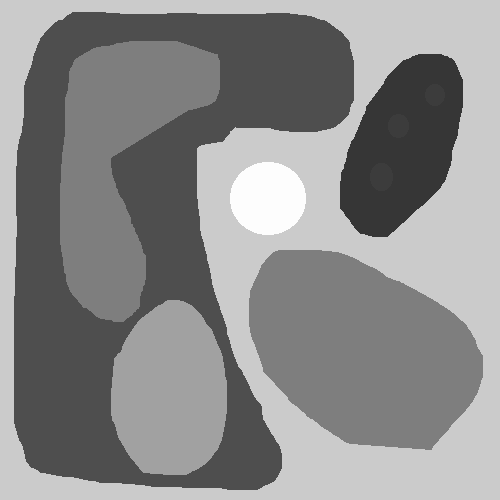
\includegraphics[scale=0.12]{leveling4}};

				\node[levelings={\imgThreeP}{\imgThreeO}{\levelingThreeB}] (leveling3) {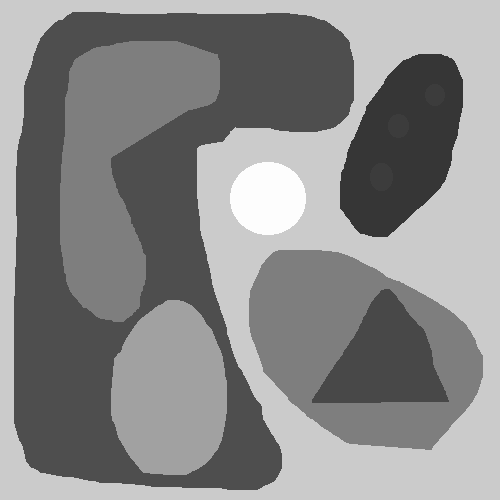
\includegraphics[scale=0.12]{leveling3}};
								
				\node[levelings={\imgTwoP}{\imgTwoO}{\levelingTwoB}] (leveling2) {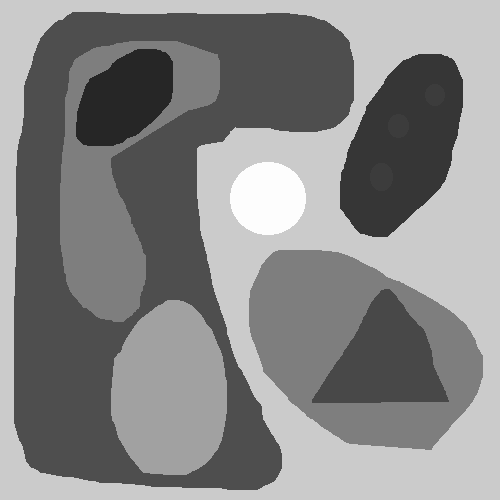
\includegraphics[scale=0.12]{leveling2}};
												
				\node[levelings={-130}{1}{\levelingOneB}] (leveling1) {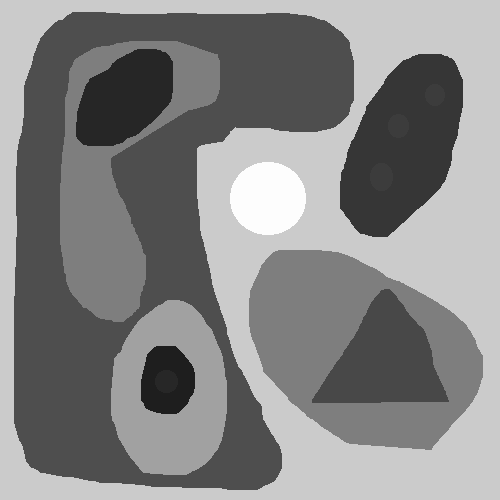
\includegraphics[scale=0.12]{leveling1}};
				
				\node[labelLeveling, opacity=\textO] at ($(leveling2)!0.5!(leveling3)$) {Espaço de escalas baseado em \textit{levelings}};
				
				% residues			

				\node[residues=\imgFourO] (residual3) at ($(leveling3)!0.5!(leveling4)$) {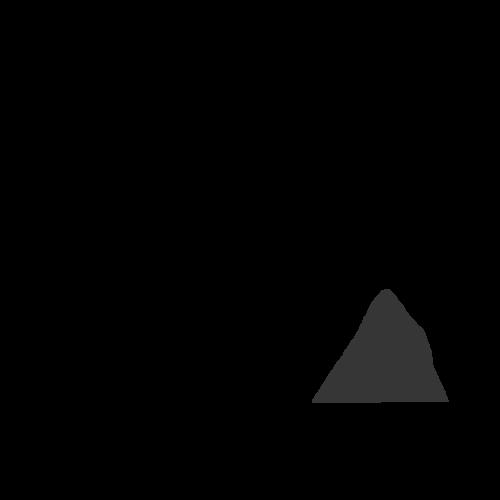
\includegraphics[scale=0.12]{residual3}};	
				
				\node[residues=\imgThreeO] (residual2) at ($(leveling2)!0.5!(leveling3)$) {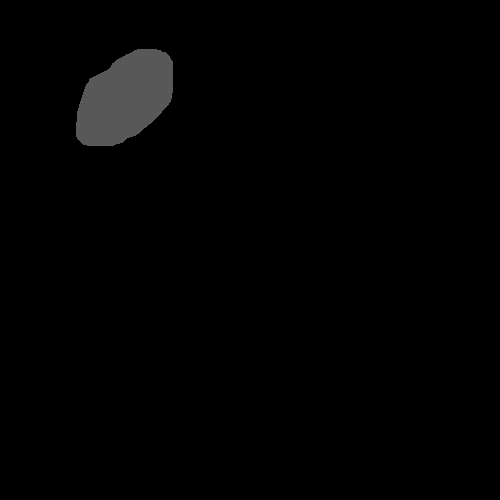
\includegraphics[scale=0.12]{residual2}};
				
				\node[label residualE=residual2, opacity=\textO]{Resíduos extraídos do espaço de escalas};				

				\node[residues=\imgTwoO] (residual1) at ($(leveling1)!0.5!(leveling2)$) {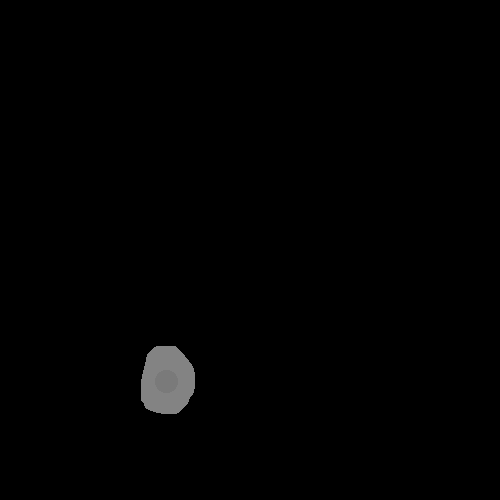
\includegraphics[scale=0.12]{residual1}};
				
				% filter and ul
				
				\node[ul={1}, opacity=\imgFourO] (residual5) at ($(residual2)!0.5!(residual3)$) {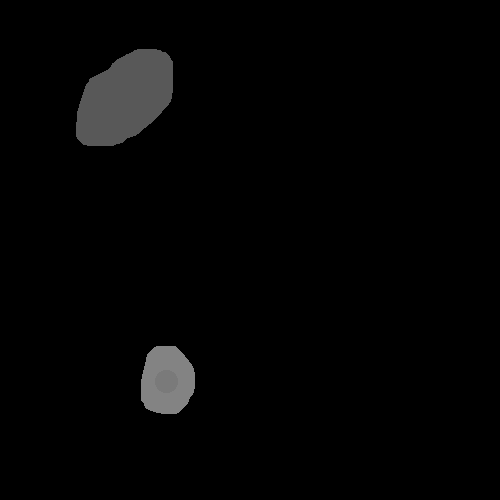
\includegraphics[scale=0.12]{residual-filtered}};
																
				\node[label residual=residual5, opacity=\textO]{\color{red}Último leveling filtrado};
				
				\node[ul={1}, opacity=\imgThreeO] (residual4) at ($(residual1)!0.5!(residual2)$) {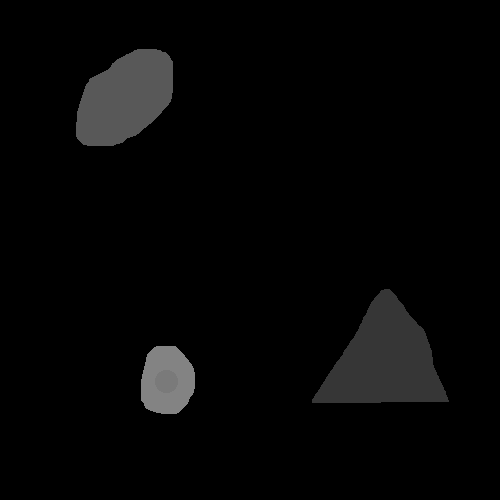
\includegraphics[scale=0.12]{residual-sup}};
												
				\node[label residual=residual4, opacity=\textO]{Último leveling};				
				
				%
				
				\ifthenelse{\i>34}{\draw[dashed](residual1) -- (residual2);}{}						

				\ifthenelse{\i>68}{\draw[dashed](residual2) -- (residual3);}{}	

	\end{tikzpicture}
	  \pgfmathtruncatemacro{\temp}{\i+1}%
	  \xdef\i{\temp}%
	  \newpage%
	}
\end{document}